\clearpage

\subsection{Opaque with 1+1 Protection}\label{ILP_Opaque_Protection}
\begin{tcolorbox}	
\begin{tabular}{p{2.75cm} p{0.2cm} p{10.5cm}} 	
\textbf{Student Name}  &:& Tiago Esteves    (October 03, 2017 - )\\
\textbf{Goal}          &:& Implement the ILP model for the opaque transport mode with 1 plus 1 protection.
\end{tabular}
\end{tcolorbox}
\vspace{11pt}

Here, in this case, we must take into account table \ref{description_opaque}, previously mentioned, in order to better understand the objective function.\\

Before carrying out the description of the objective function we must take into account the following particularity of this mode of transport:
\begin{itemize}
  \item $N_{OXC,n}$ = 0, \quad $\forall$ n
  \item $N_{EXC,n}$ = 1, \quad $\forall$ n that process traffic
\end{itemize}


\vspace{11pt}
The objective function of following the ILP is a minimization of the CAPEX through the equation \ref{Capex} where in this case for the cost of nodes we only have in consideration the electric cost \ref{Capex_Node_EXC} because of the particularity previously mentioned.
In this case the value of $P_{exc,c,n}$ is obtained by equation \ref{EXC_pexc1_opaquep} for long-reach and by the equation \ref{EXC_pexc2_opaquep} for short-reach.\\

As previously mentioned, equation \ref{EXC_pexc1_opaquep} refers to the number of long-reach ports of the electrical switch with bit-rate -1 in node n, $P_{exc,-1,n}$, i.e. the number of line ports of node n which can be calculated as

\begin{equation}
P_{exc,-1,n} = \sum_{j=1}^{N} w_{nj}
\label{EXC_pexc1_opaquep}
\end{equation}

\vspace{11pt}
where $w_{nj}$ is the number of optical channels between node $n$ and node $j$.

\vspace{11pt}
As previously mentioned, equation \ref{EXC_pexc2_opaque} refers to the number of sort-reach ports of the electrical switch with bit-rate c in node n, $P_{exc,c,n}$, i.e. the number of tributary ports with bit-rate c in node n which can be calculated as

\begin{equation}
P_{exc,c,n} = \sum_{d=1}^{N} D_{nd,c}
\label{EXC_pexc2_opaquep}
\end{equation}

\vspace{11pt}
where $D_{nd,c}$ are the client demands between nodes $n$ and $d$ with bit rate $c$.

\vspace{11pt}
In this case there is the following particularity:

\begin{itemize}
  \item When $n$=$d$ the value of client demands is always zero, i.e, $D_{nn,c}=0$
\end{itemize}


\vspace{17pt}
The objective function, to be minimized, is the expression \ref{ILPOpaque_CAPEX}.\\

$subject$ $to$
\begin{equation}
\sum_{j\textbackslash \{o\}} f_{ij}^{od} = 2  \qquad \qquad \qquad \qquad \qquad \qquad \qquad \qquad \qquad \qquad
\forall(o,d) : o < d, \forall i: i = o
\label{ILPOpaque1}
\end{equation}

This constraint are equal to the constraint \ref{ILPOpaque1_CAPEX} assuming that Z variable has the value of 2 (work and protection).

\begin{equation}
\sum_{j\textbackslash \{o\}} f_{ij}^{od} = \sum_{j\textbackslash \{d\}} f_{ji}^{od}   \qquad \qquad \qquad \qquad \qquad \qquad \qquad \qquad
\forall(o,d) : o < d, \forall i: i \neq o,d
\label{ILPOpaque2}
\end{equation}

This constraint are equal to the constraint \ref{ILPOpaque2_CAPEX}.

\begin{equation}
\sum_{j\textbackslash \{d\}} f_{ji}^{od} = 2  \qquad \qquad \qquad \qquad \qquad \qquad \qquad \qquad \qquad \qquad
\forall(o,d) : o < d, \forall i: i = d
\label{ILPOpaque3}
\end{equation}

This constraint are equal to the constraint \ref{ILPOpaque3_CAPEX} assuming that Z variable has the value of 2 (work and protection).

\begin{equation}
\sum_{o=1} \sum_{d=o+1} \left(f_{ij}^{od} + f_{ji}^{od}\right) + \sum_{c\in C} (B\left(c\right) D_{odc}\leq \tau W_{ij} G_{ij} \qquad \qquad \qquad
\forall(i,j) : i < j
\label{ILPOpaque4}
\end{equation}

This restriction is considered grooming constraint, so it means the total client traffic flows can not be greater than the capacity of optical transmission system on all links where $\tau$ is always 100.

\begin{equation}
W_{ij} \leq K_{ij} L_{ij} \qquad \qquad \qquad \qquad \qquad \qquad \qquad \qquad \qquad \qquad \qquad \qquad \forall(i,j) : i < j
\label{ILPOpaque5}
\end{equation}

This restriction concerns the capacity of the optical channels which must be less or equal to the maximum number of optical channels. For any situation the maximum number of optical channels supported by each transmission system is 100, i.e., $K_{ij}$ = 100.

\begin{equation}
\sum_{(o,d)} \left(f_{ij}^{od} + f_{ji}^{od}\right)\leq K_{ij} L_{ij} \qquad \qquad \qquad \qquad \qquad \qquad \qquad \qquad \qquad
\forall (i,j)
\label{ILPOpaqueX}
\end{equation}

This restriction answers capacity constraint problem. Then, total flows must be less or equal to the capacity of network links.
\newpage
\begin{equation}
L_{ij} , f_{ij}^{od} , f_{ji}^{od} \in \{0,1\}   \qquad \qquad \qquad \qquad \qquad \qquad \qquad \qquad
\forall(i,j) : i < j, \forall(o,d) : o < d
\label{ILPOpaque6}
\end{equation}

The number of flows per demand in this case can be zero if there are no traffic demands or one if considering working or protection traffic, in relation to the use of the link, can be zero if it is not being used or one if is being used.

\begin{equation}
W_{ij} \in \mathbb{N}  \qquad \qquad \qquad \qquad \qquad \qquad \qquad \qquad \qquad \qquad \qquad \qquad \qquad
\forall(i,j) : i < j\label{ILPOpaque7}
\end{equation}

The last constraint is just needed to ensure the number optical of channels is a positive integer values greater than zero.\\


\subsubsection{Result description}

To perform the calculations using the implementation of the models described in previous subsection it is necessary to use the MATLAB once more. \\
We already have all the necessary to obtain the CAPEX value for the reference network \ref{Reference_Network_Topology}. As described in the subsection of network traffic \ref{Reference_Network_Traffic}, we have three values of network traffic (low, medium and high traffic) so we have to obtain three different CAPEX.
The value of the CAPEX of the network will be calculated based on the costs of the equipment present in the table \ref{table_cost_ilp}.\\

It should be mentioned again that for all these final results it was necessary to take into account some restrictions, which are:
\begin{itemize}
  \item The solution is possible or impossible (we discard the case in which there is blocking).
  \item Each link only supports one transmission system.
  \item All demands have to follow the same path.
\end{itemize}

\vspace{17pt}
\textbf{Low Traffic Scenario:}\\

In this scenario we have to take into account the traffic calculated in \ref{low_traffic_scenario}. In a first phase we will show the various exiting topologies of the network. The first are the allowed topologies, physical and optical topology, the second are the logical topology for all ODUs and finally the resulting physical and optical topology.\\

\begin{figure}[h!]
\centering
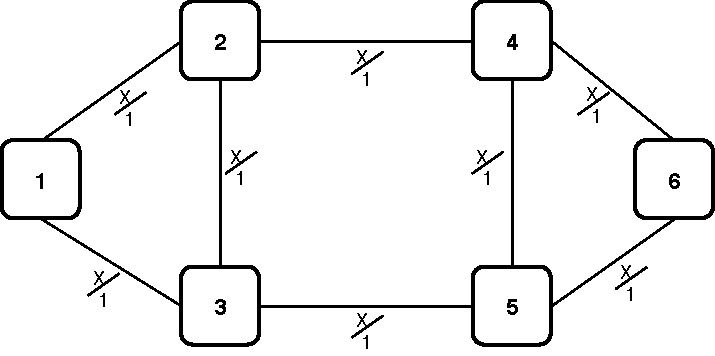
\includegraphics[width=12cm]{sdf/ilp/opaque_protection/figures/allowed_physical_topology}
\caption{Allowed Physical Topology.}
\label{allowed_physical_protectionlow}
\end{figure}

\begin{figure}[h!]
\centering
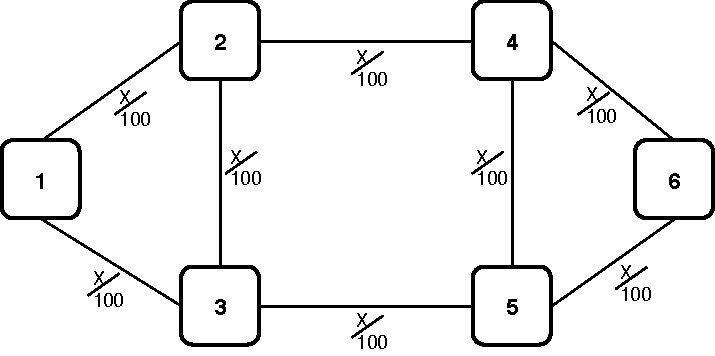
\includegraphics[width=12cm]{sdf/ilp/opaque_protection/figures/allowed_optical_topology}
\caption{Allowed Optical Topology.}
\label{allowed_optical_protectionlow}
\end{figure}

\begin{figure}[h!]
\centering
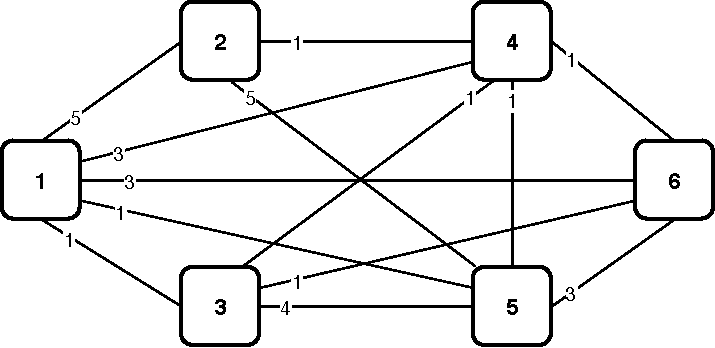
\includegraphics[width=12cm]{sdf/ilp/opaque_protection/figures/logical_topology_ODU0_low}
\caption{Logical Topology of ODU0.}
\label{logical_ODU0_protectionlow}
\end{figure}
\newpage
\begin{figure}[h!]
\centering
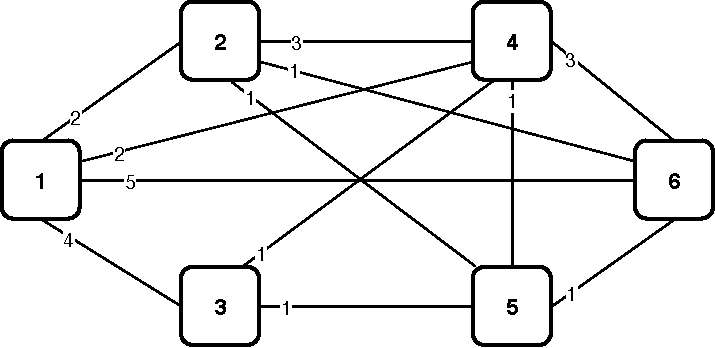
\includegraphics[width=12cm]{sdf/ilp/opaque_protection/figures/logical_topology_ODU1_low}
\caption{Logical Topology of ODU1.}
\label{logical_ODU1_protectionlow}
\end{figure}

\begin{figure}[h!]
\centering
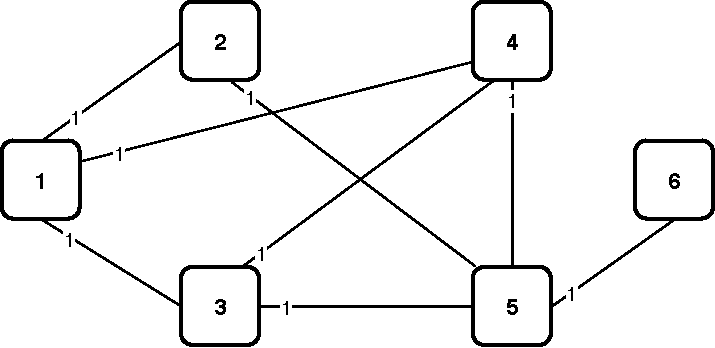
\includegraphics[width=12cm]{sdf/ilp/opaque_protection/figures/logical_topology_ODU2_low}
\caption{Logical Topology of ODU2.}
\label{logical_ODU2_protectionlow}
\end{figure}

\begin{figure}[h!]
\centering
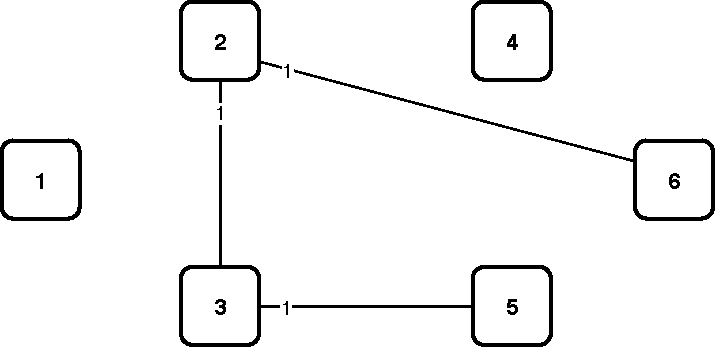
\includegraphics[width=12cm]{sdf/ilp/opaque_protection/figures/logical_topology_ODU3_low}
\caption{Logical Topology of ODU3.}
\label{logical_ODU3_protectionlow}
\end{figure}
\newpage
\begin{figure}[h!]
\centering
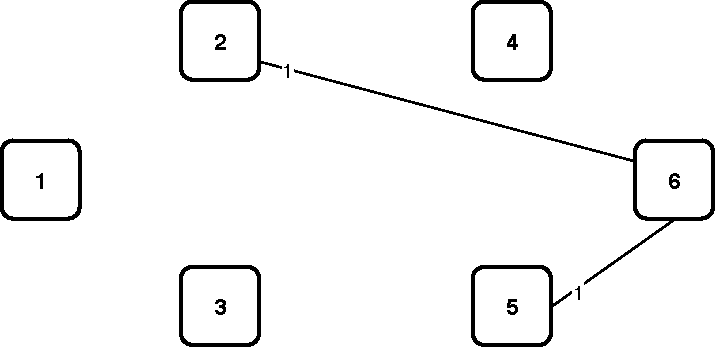
\includegraphics[width=12cm]{sdf/ilp/opaque_protection/figures/logical_topology_ODU4_low}
\caption{Logical Topology of ODU4.}
\label{logical_ODU4_protectionlow}
\end{figure}

\begin{figure}[h!]
\centering
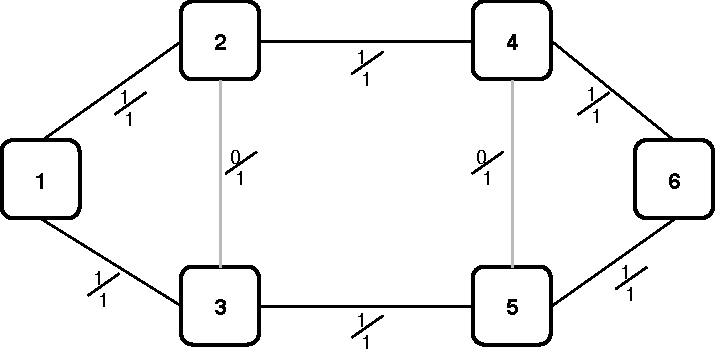
\includegraphics[width=11cm]{sdf/ilp/opaque_protection/figures/physical_topology_low}
\caption{Physical Topology.}
\label{physical_protectionlow}
\end{figure}

\begin{figure}[h!]
\centering
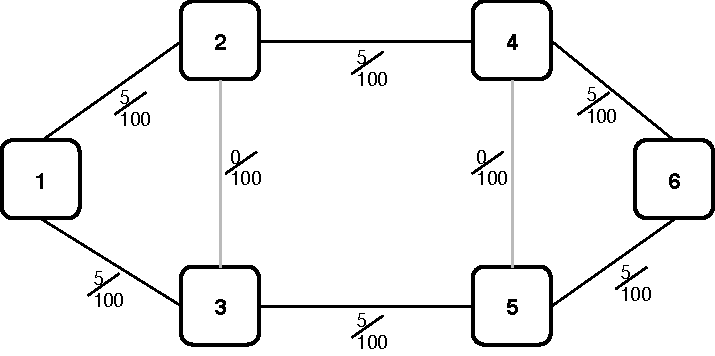
\includegraphics[width=11cm]{sdf/ilp/opaque_protection/figures/optical_topology_low}
\caption{Optical Topology.}
\label{optical_protectionlow}
\end{figure}

\newpage
\newpage
In table \ref{link_opaque_protec_ref_low} we can see the number of optical channels and the number of amplifiers for each link calculated through MatLab.\\

\begin{table}[h!]
\centering
\begin{tabular}{|| c | c | c ||}
 \hline
 \multicolumn{3}{|| c ||}{Information regarding links} \\
 \hline
 \hline
 Bidirectional Link & Optical Channels & Amplifiers\\
 \hline
 Node 1 <-> Node 2 & 5 & 4 \\
 Node 1 <-> Node 3 & 5 & 6 \\
 Node 2 <-> Node 3 & 0 & 0 \\
 Node 2 <-> Node 4 & 5 & 6 \\
 Node 3 <-> Node 5 & 5 & 8 \\
 Node 4 <-> Node 5 & 0 & 1 \\
 Node 4 <-> Node 6 & 5 & 7 \\
 Node 5 <-> Node 6 & 5 & 3 \\
 \hline
\end{tabular}
\caption{Table with information regarding links}
\label{link_opaque_protec_ref_low}
\end{table}

\vspace{11pt}
In table \ref{node_opaque_protec_ref_low}  we can see the number of connections that each node has, the number of line ports and the number of tributary ports for each node.\\

\begin{table}[h!]
\centering
\begin{tabular}{|| c | c | c | c ||}
 \hline
 \multicolumn{4}{|| c ||}{Information regarding nodes} \\
 \hline
 \hline
 Node & Resulting Nodal Degree & Line Ports & Tributary Ports\\
 \hline
 1 & 2 & 10 & 29 \\
 2 & 2 & 10 & 23 \\
 3 & 2 & 10 & 18 \\
 4 & 2 & 10 & 20 \\
 5 & 2 & 10 & 24 \\
 6 & 2 & 10 & 22 \\
\hline
\end{tabular}
\caption{Table with information regarding nodes}
\label{node_opaque_protec_ref_low}
\end{table}

\vspace{11pt}
Through the information obtained previously on the nodes we can now create tables with detailed information about each node.\\
In each table mentioned below we can see how many ports are connected to a given node and its bit rate (in relation to the line ports) and how many ports are assigned to each different bit rate (in relation to the tributary ports).\\

\begin{table}[h!]
\centering
\begin{tabular}{|| c | c | c ||}
 \hline
 \multicolumn{3}{|| c ||}{Detailed description of Node 1} \\
 \hline
 \hline
 \multirow{2}{*}{10 line ports} & 5 connect to Node 2 & \multirow{2}{*}{100 Gbits/s} \\
 & 5 connect to Node 3 & \\ \hline
\multirow{3}{*}{29 tributary ports} & 13 & ODU0 \\
 & 13 & ODU1 \\
 & 3 & ODU2 \\
\hline
\end{tabular}
\caption{Table with detailed description of node 1}
\end{table}

\begin{table}[h!]
\centering
\begin{tabular}{|| c | c | c ||}
 \hline
 \multicolumn{3}{|| c ||}{Detailed description of Node 2} \\
 \hline
 \hline
 \multirow{2}{*}{10 line ports} & 5 connect to Node 1 & \multirow{2}{*}{100 Gbits/s} \\
 & 5 connect to Node 4 & \\ \hline
\multirow{5}{*}{23 tributary ports} & 11 & ODU0 \\
 & 7 & ODU1 \\
 & 2 & ODU2 \\
 & 2 & ODU3 \\
 & 1 & ODU4 \\
\hline
\end{tabular}
\caption{Table with detailed description of node 2}
\end{table}

\newpage
\begin{table}[h!]
\centering
\begin{tabular}{|| c | c | c ||}
 \hline
 \multicolumn{3}{|| c ||}{Detailed description of Node 3} \\
 \hline
 \hline
 \multirow{2}{*}{10 line ports} & 5 connect to Node 1 & \multirow{2}{*}{100 Gbits/s}\\
 & 5 connect to Node 5 & \\ \hline
\multirow{4}{*}{18 tributary ports} & 7 & ODU0 \\
 & 6 & ODU1\\
 & 3 & ODU2\\
 & 2 & ODU3\\
\hline
\end{tabular}
\caption{Table with detailed description of node 3}
\end{table}

\begin{table}[h!]
\centering
\begin{tabular}{|| c | c | c ||}
 \hline
 \multicolumn{3}{|| c ||}{Detailed description of Node 4} \\
 \hline
 \hline
 \multirow{2}{*}{10 line ports} & 5 connect to Node 2 & \multirow{2}{*}{100 Gbits/s}\\
 & 5 connect to Node 6 & \\ \hline
\multirow{3}{*}{20 tributary ports} & 7 & ODU0 \\
 & 10 & ODU1 \\
 & 3 & ODU2 \\
\hline
\end{tabular}
\caption{Table with detailed description of node 4}
\end{table}

\begin{table}[h!]
\centering
\begin{tabular}{|| c | c | c ||}
 \hline
 \multicolumn{3}{|| c ||}{Detailed description of Node 5} \\
 \hline
 \hline
 \multirow{2}{*}{10 line ports} & 5 connect to Node 3 & \multirow{2}{*}{100 Gbits/s}\\
 & 5 connect to Node 6 & \\ \hline
\multirow{5}{*}{24 tributary ports} & 14 & ODU0 \\
 & 4 & ODU1 \\
 & 4 & ODU2 \\
 & 1 & ODU3 \\
 & 1 & ODU4 \\
\hline
\end{tabular}
\caption{Table with detailed description of node 5}
\end{table}

\begin{table}[h!]
\centering
\begin{tabular}{|| c | c | c ||}
 \hline
 \multicolumn{3}{|| c ||}{Detailed description of Node 6} \\
 \hline
 \hline
 \multirow{2}{*}{10 line ports} & 5 connect to Node 4 & \multirow{2}{*}{100 Gbits/s}\\
 &52 connect to Node 5 & \\ \hline
\multirow{5}{*}{22 tributary ports} & 8 & ODU0 \\
 & 10 & ODU1 \\
 & 1 & ODU2 \\
 & 1 & ODU3 \\
 & 2 & ODU4 \\
\hline
\end{tabular}
\caption{Table with detailed description of node 6}
\end{table}

\newpage
Now through the table \ref{scriptopaque_protec_ref_low} we can see the result of CAPEX obtained with this ILP model.\\

\begin{table}[h!]
\centering
\begin{tabular}{|| c | c | c | c | c | c | c ||}
 \hline
 \multicolumn{7}{|| c ||}{CAPEX of the Network} \\
 \hline
 \hline
 \multicolumn{3}{|| c |}{ } & Quantity & Unit Price & Cost & Total \\
 \hline
 \multirow{3}{*}{Link Cost} & \multicolumn{2}{ c |}{OLTs} & 12 & 15 000 \euro & 180 000 \euro & \multirow{3}{*}{30 452 000 \euro} \\ \cline{2-6}
 & \multicolumn{2}{ c |}{100 Gb/s Transceivers} & 60 & 5 000 \euro/Gb/s & 30 000 000 \euro & \\ \cline{2-6}
 & \multicolumn{2}{ c |}{Amplifiers} & 68 & 4 000 \euro & 272 000 \euro & \\
 \hline
 \multirow{9}{*}{Node Cost} & \multirow{7}{*}{Electrical} & EXCs & 6 & 10 000 \euro & 60 000 \euro & \multirow{9}{*}{6 062 590 \euro} \\ \cline{3-6}
 & & ODU0 Ports & 60 & 8 \euro/Gb/s & 600 \euro & \\ \cline{3-6}
 & & ODU1 Ports & 50 & 6 \euro/Gb/s & 750 \euro & \\ \cline{3-6}
 & & ODU2 Ports & 16 & 3 \euro/Gb/s & 480 \euro & \\ \cline{3-6}
 & & ODU3 Ports & 6 & 1.5 \euro/Gb/s & 360 \euro & \\ \cline{3-6}
 & & ODU4 Ports & 4 & 1 \euro/Gb/s & 400 \euro & \\ \cline{3-6}
 & & Line Ports & 60 & 1 000 \euro/Gb/s & 6 000 000 \euro & \\ \cline{2-6}
 & \multirow{2}{*}{Optical} & OXCs & 0 & 20 000 \euro & 0 \euro & \\ \cline{3-6}
 & & Ports & 0 & 2 500 \euro/porto & 0 \euro & \\
 \hline
 \multicolumn{6}{|| c |}{Total Network Cost} & 36 514 590 \euro \\
\hline
\end{tabular}
\caption{Table with detailed description of CAPEX}
\label{scriptopaque_protec_ref_low}
\end{table}

\newpage
Through the formulas mentioned below we can see how all the values of the quantity column were calculated.\\

\begin{table}[h!]
\centering
\begin{tabular}{|| c | c ||}
 \hline
 OLTs: & \(\displaystyle 2 \sum_{i=1}^{N}\sum_{j=i+1}^{N} L_{ij} \) \\ \hline
 Transceivers: & \(\displaystyle 2 \sum_{i=1}^{N}\sum_{j=i+1}^{N} W_{ij} \) \\ \hline
 Amplifiers: & \(\displaystyle \sum_{i=1}^{N}\sum_{j=i+1}^{N} N^R_{ij} L_{ij} \) \\ \hline
 EXCs: & \(\displaystyle \sum_n^N N_{EXC,n} \) \\ \hline
 ODU0: & \(\displaystyle \sum_{o=1}^{N}\sum_{d=1}^{N} D_{od,0} \) \\ \hline
 ODU1: & \(\displaystyle \sum_{o=1}^{N}\sum_{d=1}^{N} D_{od,1} \) \\ \hline
 ODU2: & \(\displaystyle \sum_{o=1}^{N}\sum_{d=1}^{N} D_{od,2} \)\\ \hline
 ODU3: & \(\displaystyle \sum_{o=1}^{N}\sum_{d=1}^{N} D_{od,3} \) \\ \hline
 ODU4: & \(\displaystyle \sum_{o=1}^{N}\sum_{d=1}^{N} D_{od,4} \) \\ \hline
 Line: & \(\displaystyle \sum_{i=1}^{N}\sum_{j=1}^{N} W_{ij} \) \\ \hline
 OXCs: & As mentioned initially this result is always zero. \\ \hline
 Ports: & Does not exist for this case then it is equal to zero. \\
 \hline
 \end{tabular}
\caption{Table with description of calculation}
\label{formulas_opaque_protec_ref_low}
\end{table}


\vspace{17pt}
Finally let's focus on the routing information. These paths are bidirectional so the path from one node to another is the same path in the opposite direction. In table \ref{path_opaque_protec_ref_low} we can see all the routing obtained for all nodes.\\
\newpage
\begin{table}[h!]
\centering
\begin{tabular}{|| c | c | c ||}
 \hline
 \multicolumn{3}{|| c ||}{Routing} \\
 \hline
 \hline
 o & d & Links \\
 \hline
 \multirow{2}{*}{1} & \multirow{2}{*}{2} & \{(1,2)\} \\
 & & \{(1,3),(3,5),(5,6),(6,4),(4,2)\} \\ \hline
 \multirow{2}{*}{1} & \multirow{2}{*}{3} & \{(1,3)\} \\
 & & \{(1,2),(2,4),(4,6),(6,5),(5,3)\} \\ \hline
 \multirow{2}{*}{1} & \multirow{2}{*}{4} & \{(1,2),(2,4)\}\\
 & & \{(1,3),(3,5),(5,6),(6,4)\} \\ \hline
 \multirow{2}{*}{1} & \multirow{2}{*}{5} & \{(1,3),(3,5)\}\\
 & & \{(1,2),(2,4),(4,6),(6,5)\} \\ \hline
 \multirow{2}{*}{1} & \multirow{2}{*}{6} & \{(1,2),(2,4),(4,6)\}\\
 & & \{(1,3),(3,5),(5,6)\} \\ \hline
 \multirow{2}{*}{2} & \multirow{2}{*}{3} & \{(2,1),(1,3)\}\\
 & & \{(2,4),(4,6),(6,5),(5,3)\} \\ \hline
 \multirow{2}{*}{2} & \multirow{2}{*}{4} & \{(2,4)\}\\
 & & \{(2,1),(1,3),(3,5),(5,6),(6,4)\} \\ \hline
 \multirow{2}{*}{2} & \multirow{2}{*}{5} & \{(2,4),(4,6),(6,5)\}\\
 & & \{(2,1),(1,3),(3,5)\} \\ \hline
 \multirow{2}{*}{2} & \multirow{2}{*}{6} & \{(2,4),(4,6)\}\\
 & & \{(2,1),(1,3),(3,5),(5,6)\} \\ \hline
 \multirow{2}{*}{3} & \multirow{2}{*}{4} & \{(3,1),(1,2),(2,4)\}\\
 & & \{(3,5),(5,6),(6,4)\} \\ \hline
 \multirow{2}{*}{3} & \multirow{2}{*}{5} & \{(3,5)\}\\
 & & \{(3,1),(1,2),(2,4),(4,6),(6,5)\} \\ \hline
 \multirow{2}{*}{3} & \multirow{2}{*}{6} & \{(3,5),(5,6)\}\\
 & & \{(3,1),(1,2),(2,4),(4,6)\} \\ \hline
 \multirow{2}{*}{4} & \multirow{2}{*}{5} & \{(4,6),(6,5)\}\\
 & & \{(4,2),(2,1),(1,3),(3,5)\} \\ \hline
 \multirow{2}{*}{4} & \multirow{2}{*}{6} & \{(4,6)\}\\
 & & \{(4,2),(2,1),(1,3),(3,5),(5,6)\} \\ \hline
 \multirow{2}{*}{5} & \multirow{2}{*}{6} & \{(5,6)\}\\
 & & \{(5,3),(3,1),(1,2),(2,4),(4,6)\} \\
 \hline
\end{tabular}
\caption{Table with description of routing}
\label{path_opaque_protec_ref_low}
\end{table}

\vspace{17pt}
\textbf{Medium Traffic Scenario:}\\

In this scenario we have to take into account the traffic calculated in \ref{medium_traffic_scenario}. In a first phase we will show the various exiting topologies of the network. The first are the allowed topologies, physical and optical topology, the second are the logical topology for all ODUs and finally the resulting physical and optical topology.

\begin{figure}[h!]
\centering
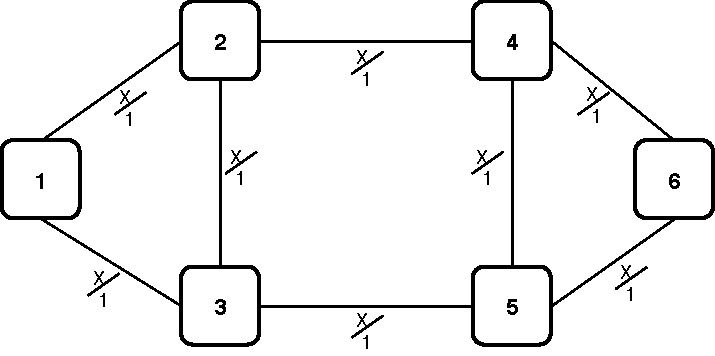
\includegraphics[width=12cm]{sdf/ilp/opaque_protection/figures/allowed_physical_topology}
\caption{Allowed Physical Topology.}
\label{allowed_physical_protectionmedium}
\end{figure}

\begin{figure}[h!]
\centering
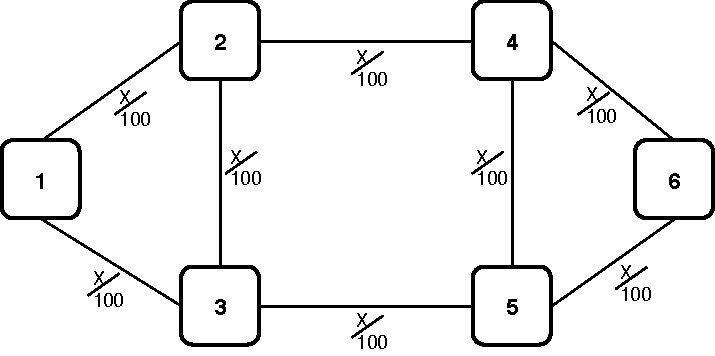
\includegraphics[width=12cm]{sdf/ilp/opaque_protection/figures/allowed_optical_topology}
\caption{Allowed Optical Topology.}
\label{allowed_optical_protectionmedium}
\end{figure}

\begin{figure}[h!]
\centering
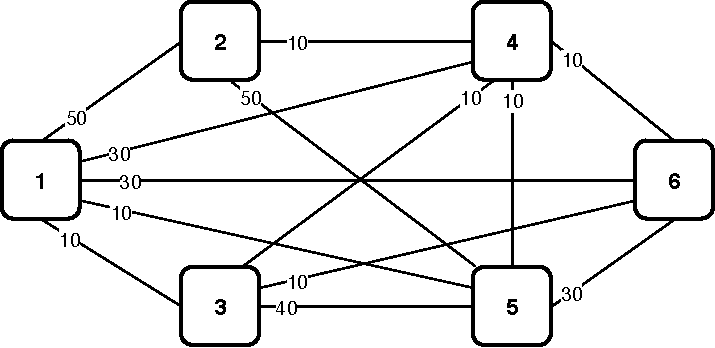
\includegraphics[width=12cm]{sdf/ilp/opaque_protection/figures/logical_topology_ODU0_medium}
\caption{Logical Topology of ODU0.}
\label{logical_ODU0_protectionmedium}
\end{figure}
\newpage
\begin{figure}[h!]
\centering
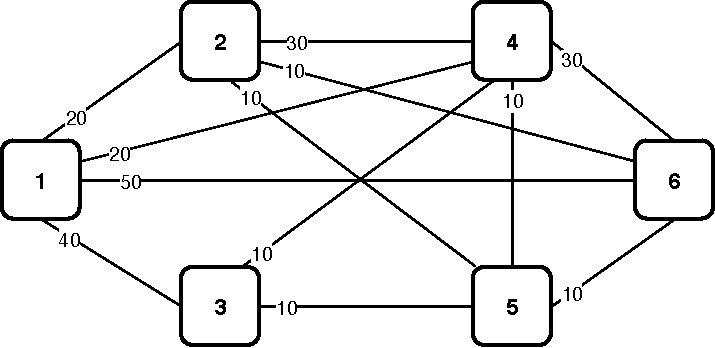
\includegraphics[width=12cm]{sdf/ilp/opaque_protection/figures/logical_topology_ODU1_medium}
\caption{Logical Topology of ODU1.}
\label{logical_ODU1_protectionmedium}
\end{figure}

\begin{figure}[h!]
\centering
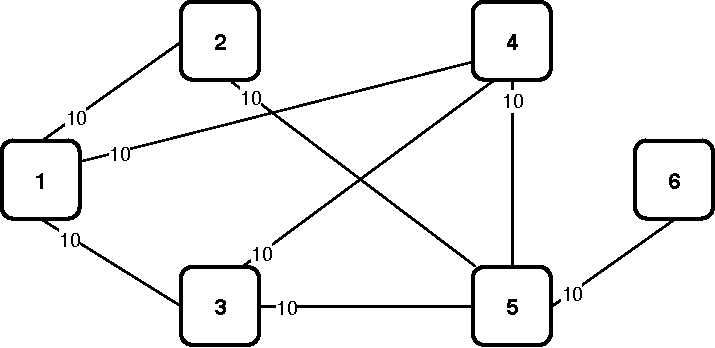
\includegraphics[width=12cm]{sdf/ilp/opaque_protection/figures/logical_topology_ODU2_medium}
\caption{Logical Topology of ODU2.}
\label{logical_ODU2_protectionmedium}
\end{figure}

\begin{figure}[h!]
\centering
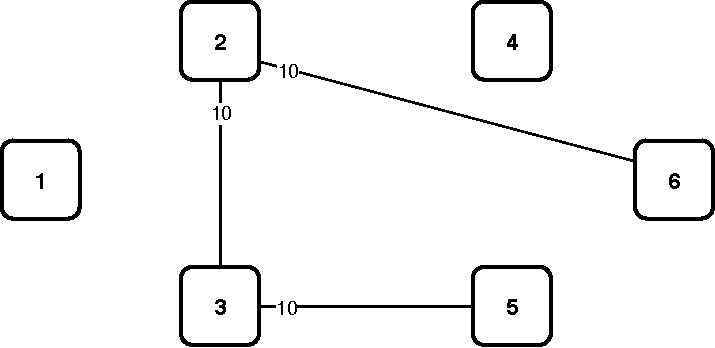
\includegraphics[width=12cm]{sdf/ilp/opaque_protection/figures/logical_topology_ODU3_medium}
\caption{Logical Topology of ODU3.}
\label{logical_ODU3_protectionmedium}
\end{figure}
\newpage
\begin{figure}[h!]
\centering
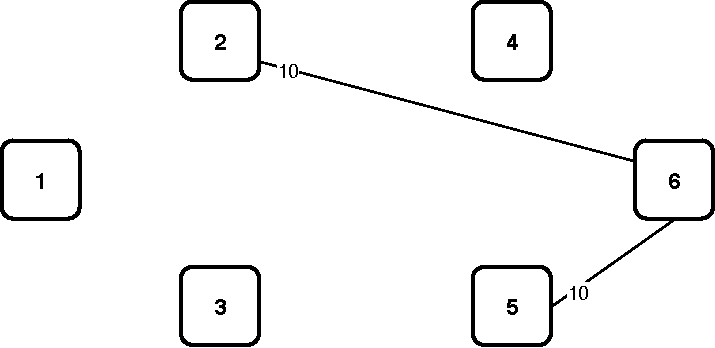
\includegraphics[width=11cm]{sdf/ilp/opaque_protection/figures/logical_topology_ODU4_medium}
\caption{Logical Topology of ODU4.}
\label{logical_ODU4_protectionmedium}
\end{figure}

\begin{figure}[h!]
\centering
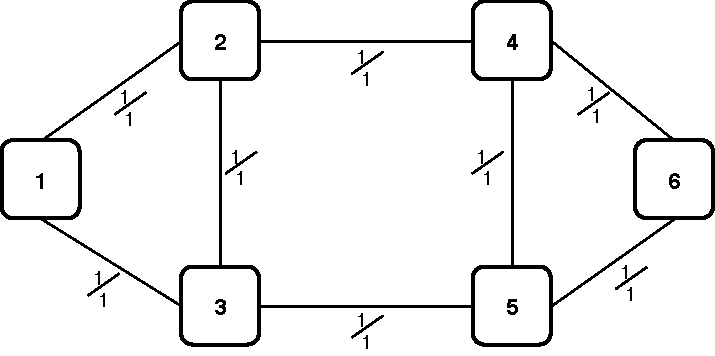
\includegraphics[width=12cm]{sdf/ilp/opaque_protection/figures/physical_topology}
\caption{Physical Topology.}
\label{physical_protectionmedium}
\end{figure}

\begin{figure}[h!]
\centering
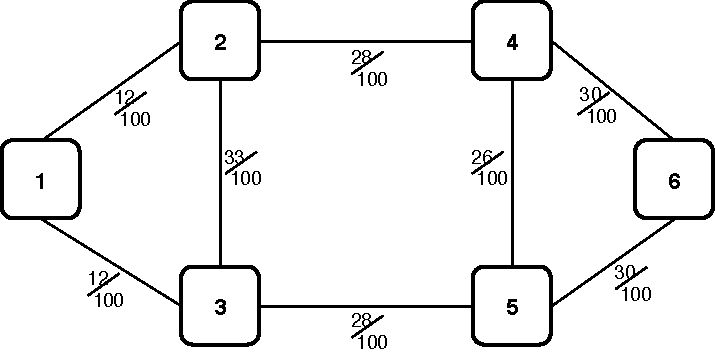
\includegraphics[width=12cm]{sdf/ilp/opaque_protection/figures/optical_topology_medium}
\caption{Optical Topology.}
\label{optical_protectionmedium}
\end{figure}

\newpage
In table \ref{link_opaque_protec_ref_medium} we can see the number of optical channels and the number of amplifiers for each link calculated through MatLab.\\

\begin{table}[h!]
\centering
\begin{tabular}{|| c | c | c ||}
 \hline
 \multicolumn{3}{|| c ||}{Information regarding links} \\
 \hline
 \hline
 Bidirectional Link & Optical Channels & Amplifiers\\
 \hline
 Node 1 <-> Node 2 & 12 & 4 \\
 Node 1 <-> Node 3 & 12 & 6 \\
 Node 2 <-> Node 3 & 33 & 0 \\
 Node 2 <-> Node 4 & 28 & 6 \\
 Node 3 <-> Node 5 & 28 & 8 \\
 Node 4 <-> Node 5 & 26 & 1 \\
 Node 4 <-> Node 6 & 30 & 7 \\
 Node 5 <-> Node 6 & 30 & 3 \\
 \hline
\end{tabular}
\caption{Table with information regarding links}
\label{link_opaque_protec_ref_medium}
\end{table}

\vspace{13pt}
In table \ref{node_opaque_protec_ref_medium} we can see the number of connections that each node has, the number of line ports and the number of tributary ports for each node.\\

\begin{table}[h!]
\centering
\begin{tabular}{|| c | c | c | c ||}
 \hline
 \multicolumn{4}{|| c ||}{Information regarding nodes} \\
 \hline
 \hline
 Node & Connections & Line Ports & Tributary Ports\\
 \hline
 1 & 2 & 24 & 290 \\
 2 & 3 & 73 & 230 \\
 3 & 3 & 73 & 180 \\
 4 & 3 & 84 & 200 \\
 5 & 3 & 84 & 240 \\
 6 & 2 & 60 & 220 \\
\hline
\end{tabular}
\caption{Table with information regarding nodes}
\label{node_opaque_protec_ref_medium}
\end{table}

\vspace{13pt}
Through the information obtained previously on the nodes we can now create tables with detailed information about each node. In each table mentioned below we can see how many ports are connected to a given node and its bit rate (in relation to the line ports) and how many ports are assigned to each different bit rate (in relation to the tributary ports).

\begin{table}[h!]
\centering
\begin{tabular}{|| c | c | c ||}
 \hline
 \multicolumn{3}{|| c ||}{Detailed description of Node 1} \\
 \hline
 \hline
\multirow{2}{*}{24 line ports} & 12 connect to Node 2 & \multirow{2}{*}{100 Gbtis/s} \\
 & 12 connect to Node 3 & \\ \hline
\multirow{3}{*}{290 tributary ports} & 130 & ODU0 \\
 & 130 & ODU1 \\
 & 30 & ODU2 \\
\hline
\end{tabular}
\caption{Table with detailed description of node 1}
\end{table}

\begin{table}[h!]
\centering
\begin{tabular}{|| c | c | c ||}
 \hline
 \multicolumn{3}{|| c ||}{Detailed description of Node 2} \\
 \hline
 \hline
 \multirow{3}{*}{73 line ports} & 12 connect to Node 1 & \multirow{3}{*}{100 Gbtis/s}\\
 & 33 connect to Node 3 & \\
 & 28 connect to Node 4 & \\ \hline
\multirow{5}{*}{230 tributary ports} & 110 & ODU0 \\
 & 70 & ODU1 \\
 & 20 & ODU2 \\
 & 20 & ODU3 \\
 & 10 & ODU4 \\
\hline
\end{tabular}
\caption{Table with detailed description of node 2}
\end{table}

\begin{table}[h!]
\centering
\begin{tabular}{|| c | c | c ||}
 \hline
 \multicolumn{3}{|| c ||}{Detailed description of Node 3} \\
 \hline
 \hline
 \multirow{3}{*}{73 line ports} & 12 connect to Node 1 & \multirow{3}{*}{100 Gbtis/s}\\
 & 33 connect to Node 2 & \\
 & 28 connect to Node 5 & \\ \hline
\multirow{4}{*}{180 tributary ports} & 70 & ODU0 \\
 & 60 & ODU1\\
 & 30 & ODU2\\
 & 20 & ODU3\\
\hline
\end{tabular}
\caption{Table with detailed description of node 3}
\end{table}

\begin{table}[h!]
\centering
\begin{tabular}{|| c | c | c ||}
 \hline
 \multicolumn{3}{|| c ||}{Detailed description of Node 4} \\
 \hline
 \hline
\multirow{3}{*}{84 line ports} & 28 connect to Node 2 & \multirow{3}{*}{100 Gbtis/s}\\
 & 26 connect to Node 5 & \\
 & 30 connect to Node 6 & \\ \hline
\multirow{3}{*}{200 tributary ports} & 70 & ODU0 \\
 & 100 & ODU1 \\
 & 30 & ODU2 \\
\hline
\end{tabular}
\caption{Table with detailed description of node 4}
\end{table}
\newpage
\begin{table}[h!]
\centering
\begin{tabular}{|| c | c | c ||}
 \hline
 \multicolumn{3}{|| c ||}{Detailed description of Node 5} \\
 \hline
 \hline
 \multirow{3}{*}{84 line ports} & 28 connect to Node 3 & \multirow{3}{*}{100 Gbtis/s} \\
 & 26 connect to Node 4 & \\
 & 30 connect to Node 6 & \\ \hline
\multirow{5}{*}{240 tributary ports} & 140 & ODU0 \\
 & 40 & ODU1 \\
 & 40 & ODU2 \\
 & 10 & ODU3 \\
 & 10 & ODU4 \\
\hline
\end{tabular}
\caption{Table with detailed description of node 5}
\end{table}

\begin{table}[h!]
\centering
\begin{tabular}{|| c | c | c ||}
 \hline
 \multicolumn{3}{|| c ||}{Detailed description of Node 6} \\
 \hline
 \hline
 \multirow{2}{*}{60 line ports} & 30 connect to Node 4 & \multirow{2}{*}{100 Gbtis/s} \\
 & 30 connect to Node 5 & \\ \hline
\multirow{5}{*}{220 tributary ports} & 80 & ODU0 \\
 & 100 & ODU1 \\
 & 10 & ODU2 \\
 & 10 & ODU3 \\
 & 20 & ODU4 \\
\hline
\end{tabular}
\caption{Table with detailed description of node 6}
\end{table}

Now through the table \ref{scriptopaque_protec_ref_medium} we can see the result of CAPEX obtained with this ILP model.

\begin{table}[h!]
\centering
\begin{tabular}{|| c | c | c | c | c | c | c ||}
 \hline
 \multicolumn{7}{|| c ||}{CAPEX of the Network} \\
 \hline
 \hline
 \multicolumn{3}{|| c |}{ } & Quantity & Unit Price & Cost & Total \\
 \hline
 \multirow{3}{*}{Link Cost} & \multicolumn{2}{ c |}{OLTs} & 16 & 15 000 \euro & 240 000 \euro & \multirow{3}{*}{199 520 000 \euro} \\ \cline{2-6}
 & \multicolumn{2}{ c |}{100 Gb/s Transceivers} & 398 & 5 000 \euro/Gb/s & 199 000 000 \euro & \\ \cline{2-6}
 & \multicolumn{2}{ c |}{Amplifiers} & 70 & 4 000 \euro & 280 000 \euro & \\
 \hline
 \multirow{9}{*}{Node Cost} & \multirow{7}{*}{Electrical} & EXCs & 6 & 10 000 \euro & 60 000 \euro & \multirow{9}{*}{39 885 900 \euro} \\ \cline{3-6}
 & & ODU0 Ports & 600 & 8 \euro/Gb/s & 6 000 \euro & \\ \cline{3-6}
 & & ODU1 Ports & 500 & 6 \euro/Gb/s & 7 500 \euro & \\ \cline{3-6}
 & & ODU2 Ports & 160 & 3 \euro/Gb/s & 4 800 \euro & \\ \cline{3-6}
 & & ODU3 Ports & 60 & 1.5 \euro/Gb/s & 3 600 \euro & \\ \cline{3-6}
 & & ODU4 Ports & 40 & 1 \euro/Gb/s & 4 000 \euro & \\ \cline{3-6}
 & & Line Ports & 398 & 1 000 \euro/Gb/s & 39 800 000 \euro & \\ \cline{2-6}
 & \multirow{2}{*}{Optical} & OXCs & 0 & 20 000 \euro & 0 \euro & \\ \cline{3-6}
 & & Ports & 0 & 2 500 \euro/porto & 0 \euro & \\
 \hline
 \multicolumn{6}{|| c |}{Total Network Cost} & 239 405 900 \euro \\
\hline
\end{tabular}
\caption{Table with detailed description of CAPEX}
\label{scriptopaque_protec_ref_medium}
\end{table}

\newpage
Through the formulas mentioned below we can see how all the values of the quantity column were calculated.\\

\begin{table}[h!]
\centering
\begin{tabular}{|| c | c ||}
 \hline
 OLTs: & \(\displaystyle 2 \sum_{i=1}^{N}\sum_{j=i+1}^{N} L_{ij} \) \\ \hline
 Transceivers: & \(\displaystyle 2 \sum_{i=1}^{N}\sum_{j=i+1}^{N} W_{ij} \) \\ \hline
 Amplifiers: & \(\displaystyle \sum_{i=1}^{N}\sum_{j=i+1}^{N} N^R_{ij} L_{ij} \) \\ \hline
 EXCs: & \(\displaystyle \sum_n^N N_{EXC,n} \) \\ \hline
 ODU0: & \(\displaystyle \sum_{o=1}^{N}\sum_{d=1}^{N} D_{od,0} \) \\ \hline
 ODU1: & \(\displaystyle \sum_{o=1}^{N}\sum_{d=1}^{N} D_{od,1} \) \\ \hline
 ODU2: & \(\displaystyle \sum_{o=1}^{N}\sum_{d=1}^{N} D_{od,2} \)\\ \hline
 ODU3: & \(\displaystyle \sum_{o=1}^{N}\sum_{d=1}^{N} D_{od,3} \) \\ \hline
 ODU4: & \(\displaystyle \sum_{o=1}^{N}\sum_{d=1}^{N} D_{od,4} \) \\ \hline
 Line: & \(\displaystyle \sum_{i=1}^{N}\sum_{j=1}^{N} W_{ij} \) \\ \hline
 OXCs: & As mentioned initially this result is always zero. \\ \hline
 Ports: & Does not exist for this case then it is equal to zero. \\
 \hline
 \end{tabular}
\caption{Table with description of calculation}
\label{formulas_opaque_protec_ref_medium}
\end{table}


\vspace{17pt}
Finally let's focus on the routing information. In table \ref{path_opaque_protec_ref_medium} we can see all the routing obtained for all nodes.\\
\newpage
\begin{table}[h!]
\centering
\begin{tabular}{|| c | c | c ||}
 \hline
 \multicolumn{3}{|| c ||}{Routing} \\
 \hline
 \hline
 o & d & Links \\
 \hline
 \multirow{2}{*}{1} & \multirow{2}{*}{2} & \{(1,2)\} \\
 & & \{(1,3),(3,2)\} \\ \hline
 \multirow{2}{*}{1} & \multirow{2}{*}{3} & \{(1,3)\} \\
 & & \{(1,2),(2,3)\} \\ \hline
 \multirow{2}{*}{1} & \multirow{2}{*}{4} & \{(1,2),(2,4)\}\\
 & & \{(1,3),(3,5),(5,4)\} \\ \hline
 \multirow{2}{*}{1} & \multirow{2}{*}{5} & \{(1,3),(3,5)\}\\
 & & \{(1,2),(2,4),(4,5)\} \\ \hline
 \multirow{2}{*}{1} & \multirow{2}{*}{6} & \{(1,2),(2,4),(4,6)\}\\
 & & \{(1,3),(3,5),(5,6)\} \\ \hline
 \multirow{2}{*}{2} & \multirow{2}{*}{3} & \{(2,3)\}\\
 & & \{(2,1),(1,3)\} \\ \hline
 \multirow{2}{*}{2} & \multirow{2}{*}{4} & \{(2,4)\}\\
 & & \{(2,3),(3,5),(5,4)\} \\ \hline
 \multirow{2}{*}{2} & \multirow{2}{*}{5} & \{(2,4),(4,5)\}\\
 & & \{(2,3),(3,5)\} \\ \hline
 \multirow{2}{*}{2} & \multirow{2}{*}{6} & \{(2,4),(4,6)\}\\
 & & \{(2,3),(3,5),(5,6)\} \\ \hline
 \multirow{2}{*}{3} & \multirow{2}{*}{4} & \{(3,2),(2,4)\}\\
 & & \{(3,5),(5,4)\} \\ \hline
 \multirow{2}{*}{3} & \multirow{2}{*}{5} & \{(3,5)\}\\
 & & \{(3,2),(2,4),(4,5)\} \\ \hline
 \multirow{2}{*}{3} & \multirow{2}{*}{6} & \{(3,5),(5,6)\}\\
 & & \{(3,2),(2,4),(4,6)\} \\ \hline
 \multirow{2}{*}{4} & \multirow{2}{*}{5} & \{(4,5)\}\\
 & & \{(4,6),(6,5)\} \\ \hline
 \multirow{2}{*}{4} & \multirow{2}{*}{6} & \{(4,6)\}\\
 & & \{(4,5),(5,6)\} \\ \hline
 \multirow{2}{*}{5} & \multirow{2}{*}{6} & \{(5,6)\}\\
 & & \{(5,4),(4,6)\} \\
 \hline
\end{tabular}
\caption{Table with description of routing}
\label{path_opaque_protec_ref_medium}
\end{table}


\vspace{17pt}
\textbf{High Traffic Scenario:}\\

In this scenario we have to take into account the traffic calculated in \ref{high_traffic_scenario}. In a first phase we will show the various exiting topologies of the network. The first are the allowed topologies, physical and optical topology, the second are the logical topology for all ODUs and finally the resulting physical and optical topology.

\begin{figure}[h!]
\centering
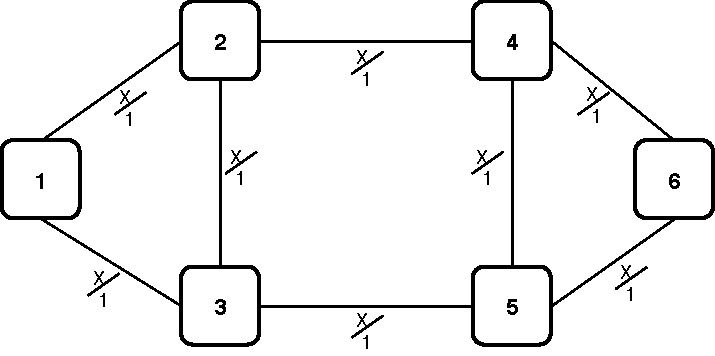
\includegraphics[width=12cm]{sdf/ilp/opaque_protection/figures/allowed_physical_topology}
\caption{Allowed Physical Topology.}
\label{allowed_physical_protectionhigh}
\end{figure}

\begin{figure}[h!]
\centering
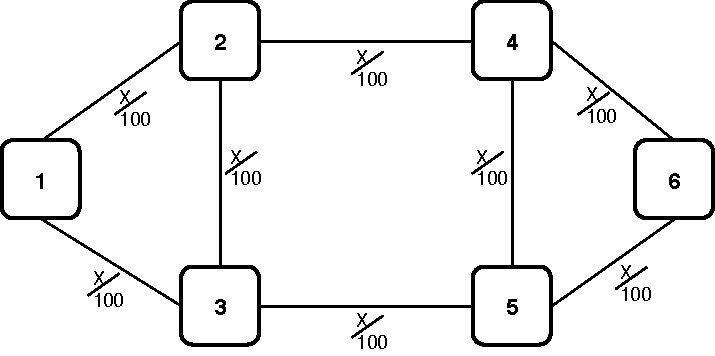
\includegraphics[width=12cm]{sdf/ilp/opaque_protection/figures/allowed_optical_topology}
\caption{Allowed Optical Topology.}
\label{allowed_optical_protectionhigh}
\end{figure}

\begin{figure}[h!]
\centering
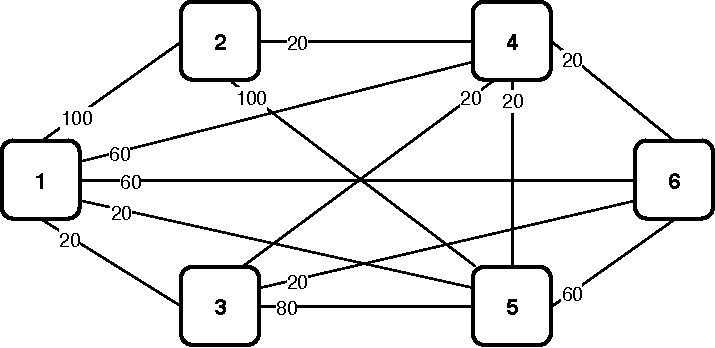
\includegraphics[width=12cm]{sdf/ilp/opaque_protection/figures/logical_topology_ODU0_high}
\caption{Logical Topology of ODU0.}
\label{logical_ODU0_protectionhigh}
\end{figure}
\newpage
\begin{figure}[h!]
\centering
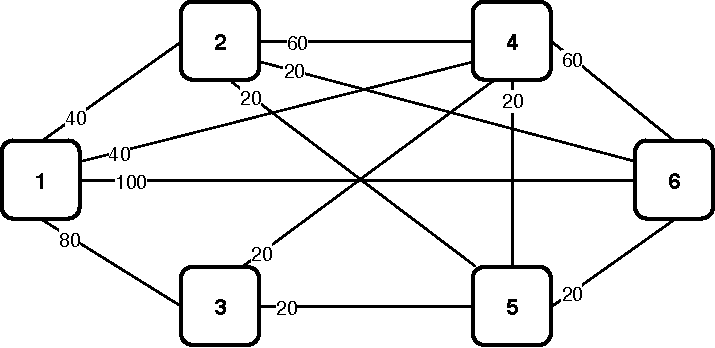
\includegraphics[width=12cm]{sdf/ilp/opaque_protection/figures/logical_topology_ODU1_high}
\caption{Logical Topology of ODU1.}
\label{logical_ODU1_protectionhigh}
\end{figure}

\begin{figure}[h!]
\centering
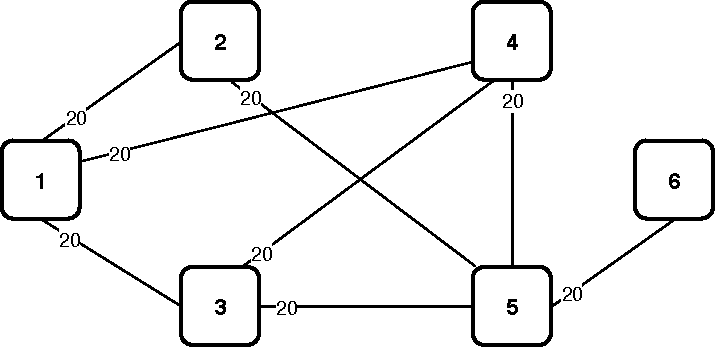
\includegraphics[width=12cm]{sdf/ilp/opaque_protection/figures/logical_topology_ODU2_high}
\caption{Logical Topology of ODU2.}
\label{logical_ODU2_protectionhigh}
\end{figure}

\begin{figure}[h!]
\centering
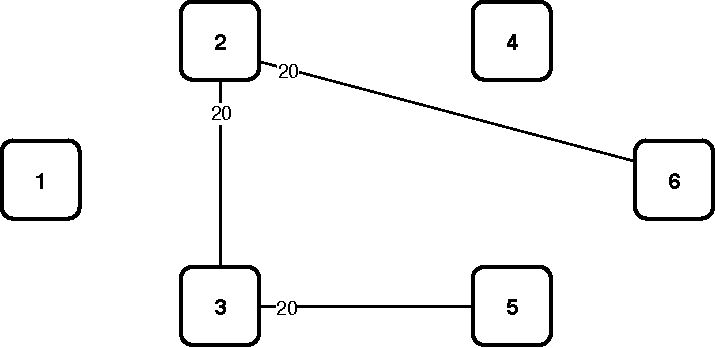
\includegraphics[width=12cm]{sdf/ilp/opaque_protection/figures/logical_topology_ODU3_high}
\caption{Logical Topology of ODU3.}
\label{logical_ODU3_protectionhigh}
\end{figure}
\newpage
\begin{figure}[h!]
\centering
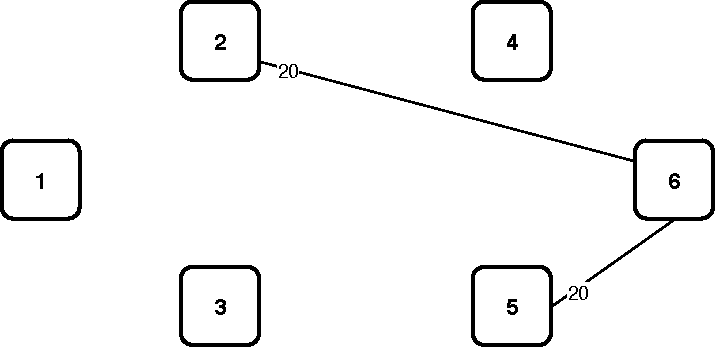
\includegraphics[width=11cm]{sdf/ilp/opaque_protection/figures/logical_topology_ODU4_high}
\caption{Logical Topology of ODU4.}
\label{logical_ODU4_protectionhigh}
\end{figure}

\begin{figure}[h!]
\centering
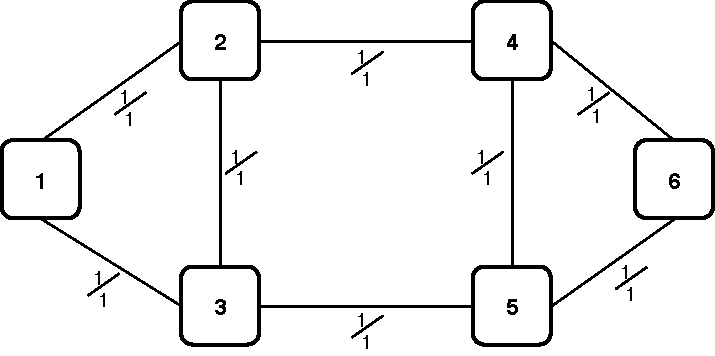
\includegraphics[width=12cm]{sdf/ilp/opaque_protection/figures/physical_topology}
\caption{Physical Topology.}
\label{physical_protectionhigh}
\end{figure}

\begin{figure}[h!]
\centering
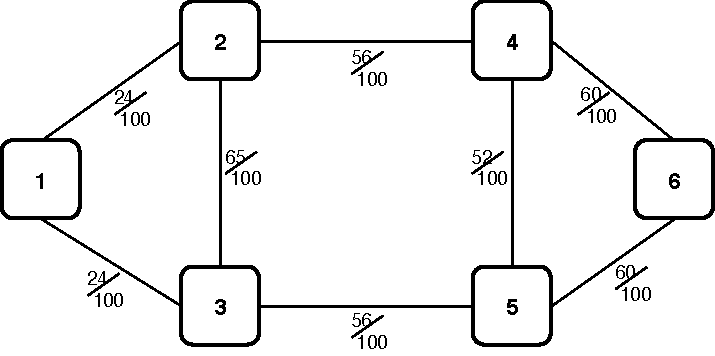
\includegraphics[width=12cm]{sdf/ilp/opaque_protection/figures/optical_topology_high}
\caption{Optical Topology.}
\label{optical_protectionhigh}
\end{figure}

\newpage
In table \ref{link_opaque_protec_ref_high} we can see the number of optical channels and the number of amplifiers for each link calculated through MatLab.\\

\begin{table}[h!]
\centering
\begin{tabular}{|| c | c | c ||}
 \hline
 \multicolumn{3}{|| c ||}{Information regarding links} \\
 \hline
 \hline
 Bidirectional Link & Optical Channels & Amplifiers\\
 \hline
 Node 1 <-> Node 2 & 24 & 4 \\
 Node 1 <-> Node 3 & 24 & 6 \\
 Node 2 <-> Node 3 & 65 & 0 \\
 Node 2 <-> Node 4 & 56 & 6 \\
 Node 3 <-> Node 5 & 56 & 8 \\
 Node 4 <-> Node 5 & 52 & 1 \\
 Node 4 <-> Node 6 & 60 & 7 \\
 Node 5 <-> Node 6 & 60 & 3 \\
 \hline
\end{tabular}
\caption{Table with information regarding links}
\label{link_opaque_protec_ref_high}
\end{table}

\vspace{13pt}
In table \ref{node_opaque_protec_ref_high} we can see the number of connections that each node has, the number of line ports and the number of tributary ports for each node.\\

\begin{table}[h!]
\centering
\begin{tabular}{|| c | c | c | c ||}
 \hline
 \multicolumn{4}{|| c ||}{Information regarding nodes} \\
 \hline
 \hline
 Node & Connections & Line Ports & Tributary Ports\\
 \hline
 1 & 2 & 48 & 580 \\
 2 & 3 & 145 & 460 \\
 3 & 3 & 145 & 360 \\
 4 & 3 & 168 & 400 \\
 5 & 3 & 168 & 480 \\
 6 & 2 & 120 & 440 \\
\hline
\end{tabular}
\caption{Table with information regarding nodes}
\label{node_opaque_protec_ref_high}
\end{table}

\vspace{13pt}
In table \ref{node_opaque_protec_ref_high} we can see the number of connections that each node has, the number of line ports and the number of tributary ports for each node.\\
In each table mentioned below we can see how many ports are connected to a given node and its bit rate (in relation to the line ports) and how many ports are assigned to each different bit rate (in relation to the tributary ports).

\begin{table}[h!]
\centering
\begin{tabular}{|| c | c | c ||}
 \hline
 \multicolumn{3}{|| c ||}{Detailed description of Node 1} \\
 \hline
 \hline
\multirow{2}{*}{48 line ports} & 24 connect to Node 2 & \multirow{2}{*}{100 Gbtis/s} \\
 & 24 connect to Node 3 & \\ \hline
\multirow{3}{*}{580 tributary ports} & 260 & ODU0 \\
 & 260 & ODU1 \\
 & 60 & ODU2 \\
\hline
\end{tabular}
\caption{Table with detailed description of node 1}
\end{table}

\begin{table}[h!]
\centering
\begin{tabular}{|| c | c | c ||}
 \hline
 \multicolumn{3}{|| c ||}{Detailed description of Node 2} \\
 \hline
 \hline
 \multirow{3}{*}{145 line ports} & 24 connect to Node 1 & \multirow{3}{*}{100 Gbtis/s}\\
 & 65 connect to Node 3 & \\
 & 56 connect to Node 4 & \\ \hline
\multirow{5}{*}{460 tributary ports} & 220 & ODU0 \\
 & 140 & ODU1 \\
 & 40 & ODU2 \\
 & 40 & ODU3 \\
 & 20 & ODU4 \\
\hline
\end{tabular}
\caption{Table with detailed description of node 2}
\end{table}

\newpage
\begin{table}[h!]
\centering
\begin{tabular}{|| c | c | c ||}
 \hline
 \multicolumn{3}{|| c ||}{Detailed description of Node 3} \\
 \hline
 \hline
 \multirow{3}{*}{145 line ports} & 24 connect to Node 1 & \multirow{3}{*}{100 Gbtis/s}\\
 & 65 connect to Node 2 & \\
 & 56 connect to Node 5 & \\ \hline
\multirow{4}{*}{360 tributary ports} & 140 & ODU0 \\
 & 120 & ODU1\\
 & 60 & ODU2\\
 & 40 & ODU3\\
\hline
\end{tabular}
\caption{Table with detailed description of node 3}
\end{table}

\begin{table}[h!]
\centering
\begin{tabular}{|| c | c | c ||}
 \hline
 \multicolumn{3}{|| c ||}{Detailed description of Node 4} \\
 \hline
 \hline
\multirow{3}{*}{168 line ports} & 56 connect to Node 2 & \multirow{3}{*}{100 Gbtis/s}\\
 & 52 connect to Node 5 & \\
 & 60 connect to Node 6 & \\ \hline
\multirow{3}{*}{400 tributary ports} & 140 & ODU0 \\
 & 200 & ODU1 \\
 & 60 & ODU2 \\
\hline
\end{tabular}
\caption{Table with detailed description of node 4}
\end{table}

\begin{table}[h!]
\centering
\begin{tabular}{|| c | c | c ||}
 \hline
 \multicolumn{3}{|| c ||}{Detailed description of Node 5} \\
 \hline
 \hline
 \multirow{3}{*}{168 line ports} & 56 connect to Node 3 & \multirow{3}{*}{100 Gbtis/s} \\
 & 52 connect to Node 4 & \\
 & 60 connect to Node 6 & \\ \hline
\multirow{5}{*}{480 tributary ports} & 280 & ODU0 \\
 & 80 & ODU1 \\
 & 80 & ODU2 \\
 & 20 & ODU3 \\
 & 20 & ODU4 \\
\hline
\end{tabular}
\caption{Table with detailed description of node 5}
\end{table}

\newpage
\begin{table}[h!]
\centering
\begin{tabular}{|| c | c | c ||}
 \hline
 \multicolumn{3}{|| c ||}{Detailed description of Node 6} \\
 \hline
 \hline
 \multirow{2}{*}{120 line ports} & 60 connect to Node 4 & \multirow{2}{*}{100 Gbtis/s} \\
 & 60 connect to Node 5 & \\ \hline
\multirow{5}{*}{440 tributary ports} & 160 & ODU0 \\
 & 200 & ODU1 \\
 & 20 & ODU2 \\
 & 20 & ODU3 \\
 & 40 & ODU4 \\
\hline
\end{tabular}
\caption{Table with detailed description of node 6}
\end{table}

Now through the table \ref{scriptopaque_protec_ref_high} we can see the result of CAPEX obtained with this ILP model.

\begin{table}[h!]
\centering
\begin{tabular}{|| c | c | c | c | c | c | c ||}
 \hline
 \multicolumn{7}{|| c ||}{CAPEX of the Network} \\
 \hline
 \hline
 \multicolumn{3}{|| c |}{ } & Quantity & Unit Price & Cost & Total \\
 \hline
 \multirow{3}{*}{Link Cost} & \multicolumn{2}{ c |}{OLTs} & 16 & 15 000 \euro & 240 000 \euro & \multirow{3}{*}{397 520 000 \euro} \\ \cline{2-6}
 & \multicolumn{2}{ c |}{100 Gb/s Transceivers} & 794 & 5 000 \euro/Gb/s & 397 000 000 \euro & \\ \cline{2-6}
 & \multicolumn{2}{ c |}{Amplifiers} & 70 & 4 000 \euro & 280 000 \euro & \\
 \hline
 \multirow{9}{*}{Node Cost} & \multirow{7}{*}{Electrical} & EXCs & 6 & 10 000 \euro & 60 000 \euro & \multirow{9}{*}{79 511 800 \euro} \\ \cline{3-6}
 & & ODU0 Ports & 1 200 & 8 \euro/Gb/s & 12 000 \euro & \\ \cline{3-6}
 & & ODU1 Ports & 1 000 & 6 \euro/Gb/s & 15 000 \euro & \\ \cline{3-6}
 & & ODU2 Ports & 320 & 3 \euro/Gb/s & 9 600 \euro & \\ \cline{3-6}
 & & ODU3 Ports & 120 & 1.5 \euro/Gb/s & 7 200 \euro & \\ \cline{3-6}
 & & ODU4 Ports & 80 & 1 \euro/Gb/s & 8 000 \euro & \\ \cline{3-6}
 & & Line Ports & 794 & 1 000 \euro/Gb/s & 79 400 000 \euro & \\ \cline{2-6}
 & \multirow{2}{*}{Optical} & OXCs & 0 & 20 000 \euro & 0 \euro & \\ \cline{3-6}
 & & Ports & 0 & 2 500 \euro/porto & 0 \euro & \\
 \hline
 \multicolumn{6}{|| c |}{Total Network Cost} & 477 031 800 \euro \\
\hline
\end{tabular}
\caption{Table with detailed description of CAPEX}
\label{scriptopaque_protec_ref_high}
\end{table}

\newpage
Through the formulas mentioned below we can see how all the values of the quantity column were calculated.\\

\begin{table}[h!]
\centering
\begin{tabular}{|| c | c ||}
 \hline
 OLTs: & \(\displaystyle 2 \sum_{i=1}^{N}\sum_{j=i+1}^{N} L_{ij} \) \\ \hline
 Transceivers: & \(\displaystyle 2 \sum_{i=1}^{N}\sum_{j=i+1}^{N} W_{ij} \) \\ \hline
 Amplifiers: & \(\displaystyle \sum_{i=1}^{N}\sum_{j=i+1}^{N} N^R_{ij} L_{ij} \) \\ \hline
 EXCs: & \(\displaystyle \sum_n^N N_{EXC,n} \) \\ \hline
 ODU0: & \(\displaystyle \sum_{o=1}^{N}\sum_{d=1}^{N} D_{od,0} \) \\ \hline
 ODU1: & \(\displaystyle \sum_{o=1}^{N}\sum_{d=1}^{N} D_{od,1} \) \\ \hline
 ODU2: & \(\displaystyle \sum_{o=1}^{N}\sum_{d=1}^{N} D_{od,2} \)\\ \hline
 ODU3: & \(\displaystyle \sum_{o=1}^{N}\sum_{d=1}^{N} D_{od,3} \) \\ \hline
 ODU4: & \(\displaystyle \sum_{o=1}^{N}\sum_{d=1}^{N} D_{od,4} \) \\ \hline
 Line: & \(\displaystyle \sum_{i=1}^{N}\sum_{j=1}^{N} W_{ij} \) \\ \hline
 OXCs: & As mentioned initially this result is always zero. \\ \hline
 Ports: & Does not exist for this case then it is equal to zero. \\
 \hline
 \end{tabular}
\caption{Table with description of calculation}
\label{formulas_opaque_protec_ref_high}
\end{table}


\vspace{17pt}
Finally let's focus on the routing information. These paths are bidirectional so the path from one node to another is the same path in the opposite direction. In table \ref{path_opaque_protec_ref_high} we can see all the routing obtained for all nodes.\\
\newpage
\begin{table}[h!]
\centering
\begin{tabular}{|| c | c | c ||}
 \hline
 \multicolumn{3}{|| c ||}{Routing} \\
 \hline
 \hline
 o & d & Links \\
 \hline
 \multirow{2}{*}{1} & \multirow{2}{*}{2} & \{(1,2)\} \\
 & & \{(1,3),(3,2)\} \\ \hline
 \multirow{2}{*}{1} & \multirow{2}{*}{3} & \{(1,3)\} \\
 & & \{(1,2),(2,3)\} \\ \hline
 \multirow{2}{*}{1} & \multirow{2}{*}{4} & \{(1,2),(2,4)\}\\
 & & \{(1,3),(3,5),(5,4)\} \\ \hline
 \multirow{2}{*}{1} & \multirow{2}{*}{5} & \{(1,3),(3,5)\}\\
 & & \{(1,2),(2,4),(4,5)\} \\ \hline
 \multirow{2}{*}{1} & \multirow{2}{*}{6} & \{(1,2),(2,4),(4,6)\}\\
 & & \{(1,3),(3,5),(5,6)\} \\ \hline
 \multirow{2}{*}{2} & \multirow{2}{*}{3} & \{(2,3)\}\\
 & & \{(2,1),(1,3)\} \\ \hline
 \multirow{2}{*}{2} & \multirow{2}{*}{4} & \{(2,4)\}\\
 & & \{(2,3),(3,5),(5,4)\} \\ \hline
 \multirow{2}{*}{2} & \multirow{2}{*}{5} & \{(2,4),(4,5)\}\\
 & & \{(2,3),(3,5)\} \\ \hline
 \multirow{2}{*}{2} & \multirow{2}{*}{6} & \{(2,4),(4,6)\}\\
 & & \{(2,3),(3,5),(5,6)\} \\ \hline
 \multirow{2}{*}{3} & \multirow{2}{*}{4} & \{(3,2),(2,4)\}\\
 & & \{(3,5),(5,4)\} \\ \hline
 \multirow{2}{*}{3} & \multirow{2}{*}{5} & \{(3,5)\}\\
 & & \{(3,2),(2,4),(4,5)\} \\ \hline
 \multirow{2}{*}{3} & \multirow{2}{*}{6} & \{(3,5),(5,6)\}\\
 & & \{(3,2),(2,4),(4,6)\} \\ \hline
 \multirow{2}{*}{4} & \multirow{2}{*}{5} & \{(4,5)\}\\
 & & \{(4,6),(6,5)\} \\ \hline
 \multirow{2}{*}{4} & \multirow{2}{*}{6} & \{(4,6)\}\\
 & & \{(4,5),(5,6)\} \\ \hline
 \multirow{2}{*}{5} & \multirow{2}{*}{6} & \{(5,6)\}\\
 & & \{(5,4),(4,6)\} \\
 \hline
\end{tabular}
\caption{Table with description of routing}
\label{path_opaque_protec_ref_high}
\end{table}


